\documentclass[11pt]{article}
\usepackage[margin=1in]{geometry}
\usepackage{tikz}
\usetikzlibrary{shapes.geometric, arrows.meta, positioning, fit, backgrounds, calc}
\usepackage{enumitem}

% ── Style Definitions ──
\tikzset{
  startstop/.style={rectangle, rounded corners=6pt, minimum width=2.4cm, minimum height=0.8cm,
    text centered, draw=black!70, fill=black!8, font=\small\bfseries},
  process/.style={rectangle, minimum width=2.8cm, minimum height=0.8cm,
    text centered, draw=blue!60, fill=blue!8, font=\small},
  decision/.style={diamond, aspect=2.2, minimum width=2cm,
    text centered, draw=orange!70, fill=orange!8, font=\small},
  io/.style={trapezium, trapezium left angle=70, trapezium right angle=110,
    minimum width=2.2cm, minimum height=0.7cm,
    text centered, draw=green!60!black, fill=green!8, font=\small},
  data/.style={rectangle, rounded corners=3pt, minimum width=2.2cm, minimum height=0.7cm,
    text centered, draw=purple!60, fill=purple!8, font=\small},
  arr/.style={-{Stealth[length=6pt]}, thick, draw=black!60},
  darr/.style={-{Stealth[length=6pt]}, thick, draw=red!60, dashed},
  group/.style={draw=gray!40, dashed, rounded corners=8pt, inner sep=10pt, fill=gray!3},
}

\title{\textbf{MagicBaton} --- System Flowcharts}
\author{}
\date{}

\begin{document}
\maketitle
\thispagestyle{empty}

% ════════════════════════════════════════════
% 1. System Architecture
% ════════════════════════════════════════════
\section{System Architecture Overview}

\begin{center}
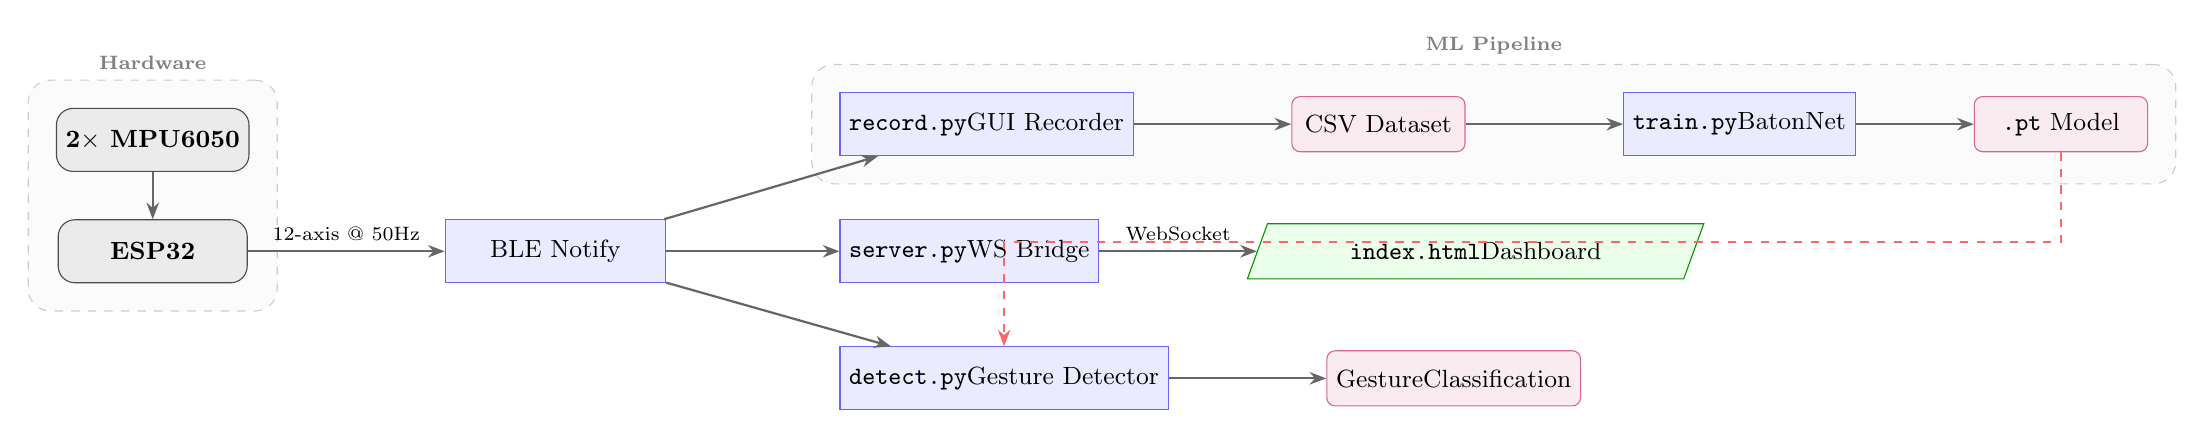
\begin{tikzpicture}[node distance=1.6cm and 2.2cm]
  % Hardware
  \node[startstop] (imu) {2$\times$ MPU6050};
  \node[startstop, below=0.6cm of imu] (esp) {ESP32};

  % Communication
  \node[process, right=2.5cm of esp] (ble) {BLE Notify};

  % Software branches
  \node[process, above right=0.8cm and 2.2cm of ble] (record) {\texttt{record.py}\\GUI Recorder};
  \node[process, right=2.2cm of ble] (server) {\texttt{server.py}\\WS Bridge};
  \node[process, below right=0.8cm and 2.2cm of ble] (detect) {\texttt{detect.py}\\Gesture Detector};

  % Outputs
  \node[data, right=2cm of record] (csv) {CSV Dataset};
  \node[process, right=2cm of csv] (train) {\texttt{train.py}\\BatonNet};
  \node[data, right=1.5cm of train] (model) {\texttt{.pt} Model};

  \node[io, right=2cm of server] (html) {\texttt{index.html}\\Dashboard};

  \node[data, right=2cm of detect] (gesture) {Gesture\\Classification};

  % Arrows
  \draw[arr] (imu) -- (esp);
  \draw[arr] (esp) -- node[above, font=\scriptsize]{12-axis @ 50Hz} (ble);
  \draw[arr] (ble) -- (record);
  \draw[arr] (ble) -- (server);
  \draw[arr] (ble) -- (detect);
  \draw[arr] (record) -- (csv);
  \draw[arr] (csv) -- (train);
  \draw[arr] (train) -- (model);
  \draw[darr] (model) -- ++(0,-1.5) -| (detect);
  \draw[arr] (server) -- node[above, font=\scriptsize]{WebSocket} (html);
  \draw[arr] (detect) -- (gesture);

  % Groups
  \begin{scope}[on background layer]
    \node[group, fit=(imu)(esp), label={[font=\scriptsize\bfseries, gray]above:Hardware}] {};
    \node[group, fit=(record)(csv)(train)(model), label={[font=\scriptsize\bfseries, gray]above:ML Pipeline}] {};
  \end{scope}
\end{tikzpicture}
\end{center}

% ════════════════════════════════════════════
% 2. Beat Detection & BPM
% ════════════════════════════════════════════
\section{Beat Detection \& BPM Estimation}

\begin{center}
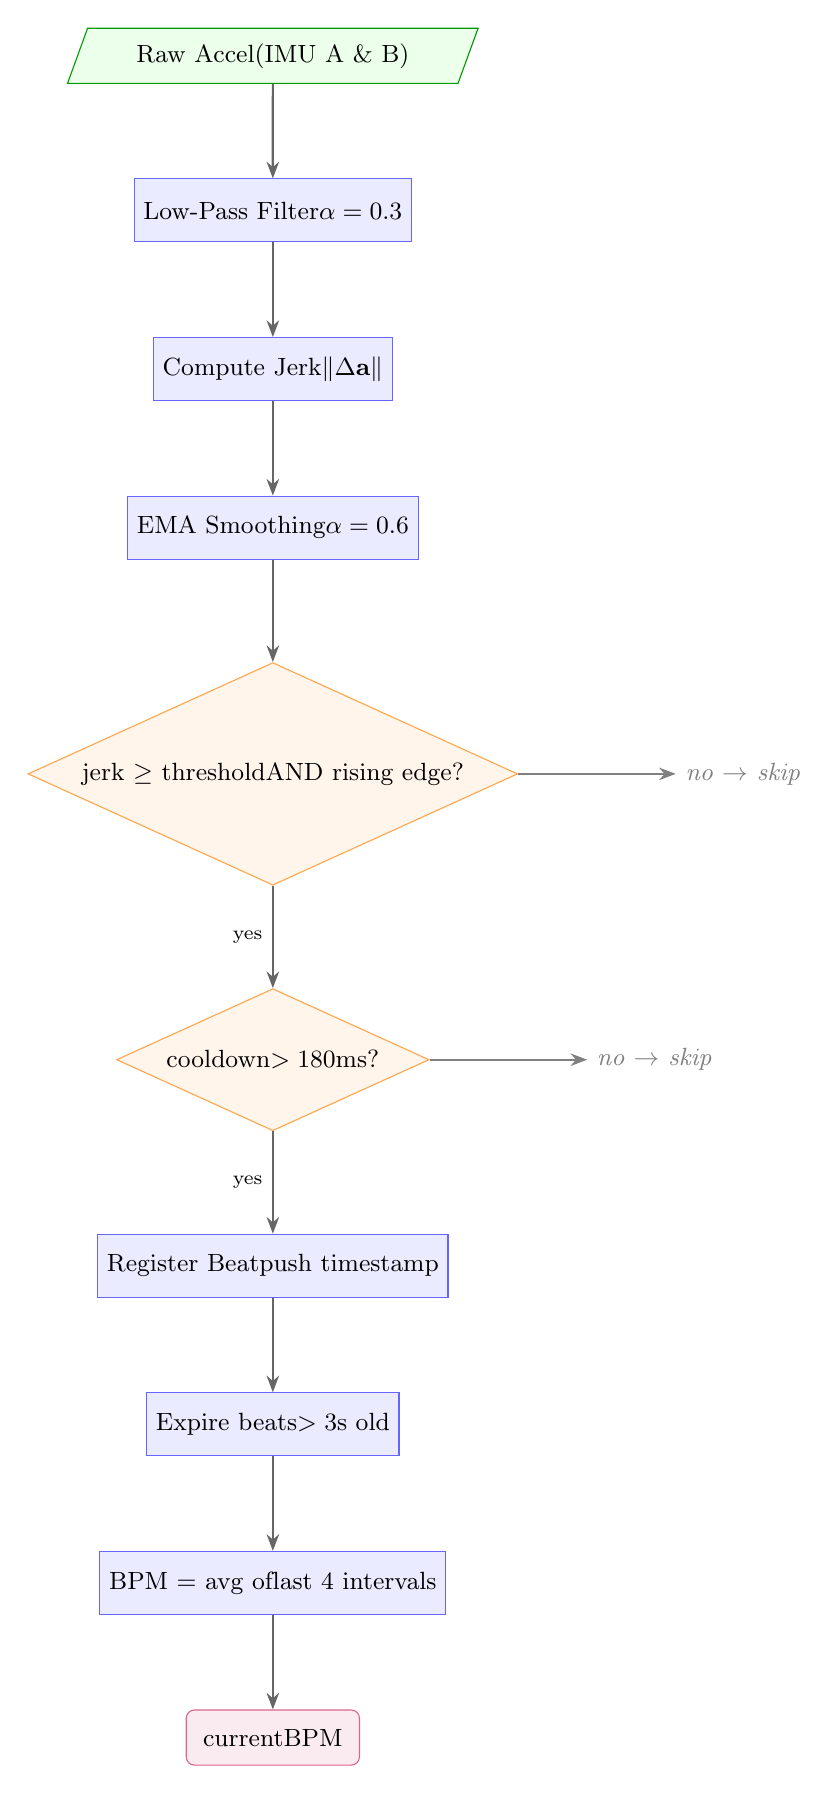
\begin{tikzpicture}[node distance=1.2cm]
  \node[io] (raw) {Raw Accel\\(IMU A \& B)};
  \node[process, below=of raw] (lp) {Low-Pass Filter\\$\alpha = 0.3$};
  \node[process, below=of lp] (jerk) {Compute Jerk\\$\|\Delta \mathbf{a}\|$};
  \node[process, below=of jerk] (smooth) {EMA Smoothing\\$\alpha = 0.6$};
  \node[decision, below=1.3cm of smooth] (thresh) {jerk $\geq$ threshold\\AND rising edge?};
  \node[decision, below=1.3cm of thresh] (cd) {cooldown\\$> 180$ms?};
  \node[process, below=1.3cm of cd] (beat) {Register Beat\\push timestamp};
  \node[process, below=of beat] (expire) {Expire beats\\$> 3$s old};
  \node[process, below=of expire] (bpm) {BPM = avg of\\last 4 intervals};
  \node[data, below=of bpm] (out) {currentBPM};

  % Side: no
  \node[right=2cm of thresh, font=\small\itshape, gray] (no1) {no $\rightarrow$ skip};
  \node[right=2cm of cd, font=\small\itshape, gray] (no2) {no $\rightarrow$ skip};

  \draw[arr] (raw) -- (lp);
  \draw[arr] (lp) -- (jerk);
  \draw[arr] (jerk) -- (smooth);
  \draw[arr] (smooth) -- (thresh);
  \draw[arr] (thresh) -- node[left, font=\scriptsize]{yes} (cd);
  \draw[arr] (cd) -- node[left, font=\scriptsize]{yes} (beat);
  \draw[arr] (beat) -- (expire);
  \draw[arr] (expire) -- (bpm);
  \draw[arr] (bpm) -- (out);
  \draw[arr, gray] (thresh) -- (no1);
  \draw[arr, gray] (cd) -- (no2);
\end{tikzpicture}
\end{center}

% ════════════════════════════════════════════
% 3. MIDI Tempo Sync
% ════════════════════════════════════════════
\section{MIDI Player \& Tempo Synchronization}

\begin{center}
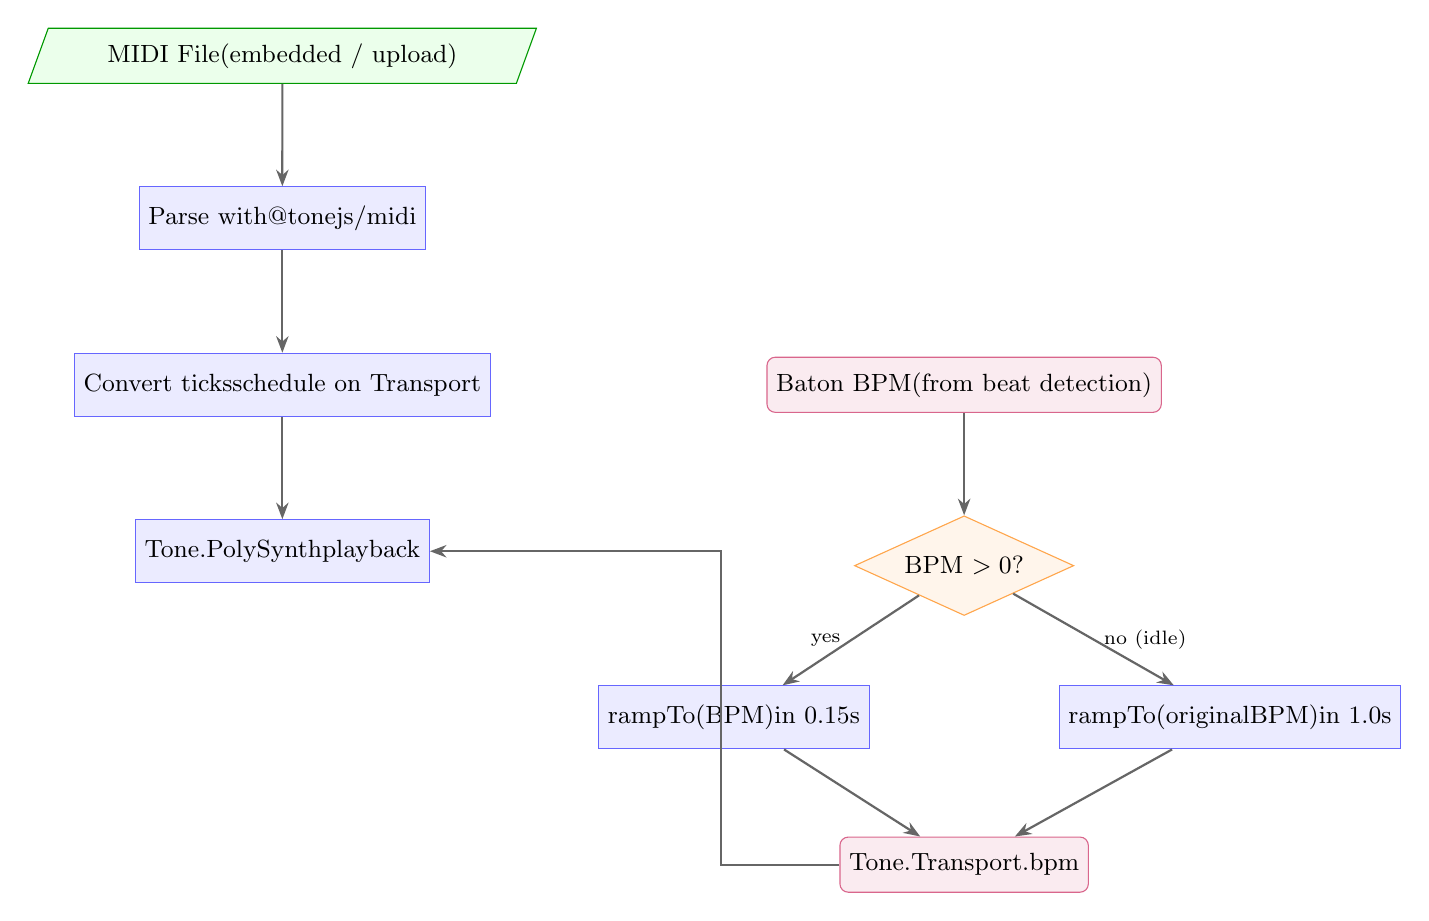
\begin{tikzpicture}[node distance=1.3cm]
  \node[io] (file) {MIDI File\\(embedded / upload)};
  \node[process, below=of file] (parse) {Parse with\\@tonejs/midi};
  \node[process, below=of parse] (schedule) {Convert ticks\\schedule on Transport};
  \node[process, below=of schedule] (synth) {Tone.PolySynth\\playback};
  \node[data, right=3.5cm of schedule] (baton) {Baton BPM\\(from beat detection)};
  \node[decision, below=1.3cm of baton] (active) {BPM $> 0$?};
  \node[process, below left=1.2cm and 0.5cm of active] (ramp) {rampTo(BPM)\\in 0.15s};
  \node[process, below right=1.2cm and 0.5cm of active] (reset) {rampTo(originalBPM)\\in 1.0s};
  \node[data, below=2.8cm of active] (transport) {Tone.Transport.bpm};

  \draw[arr] (file) -- (parse);
  \draw[arr] (parse) -- (schedule);
  \draw[arr] (schedule) -- (synth);
  \draw[arr] (baton) -- (active);
  \draw[arr] (active) -- node[left, font=\scriptsize]{yes} (ramp);
  \draw[arr] (active) -- node[right, font=\scriptsize]{no (idle)} (reset);
  \draw[arr] (ramp) -- (transport);
  \draw[arr] (reset) -- (transport);
  \draw[arr] (transport.west) -- ++(-1.5,0) |- (synth.east);
\end{tikzpicture}
\end{center}

% ════════════════════════════════════════════
% 4. Gesture Detection
% ════════════════════════════════════════════
\section{Real-Time Gesture Detection}

\begin{center}
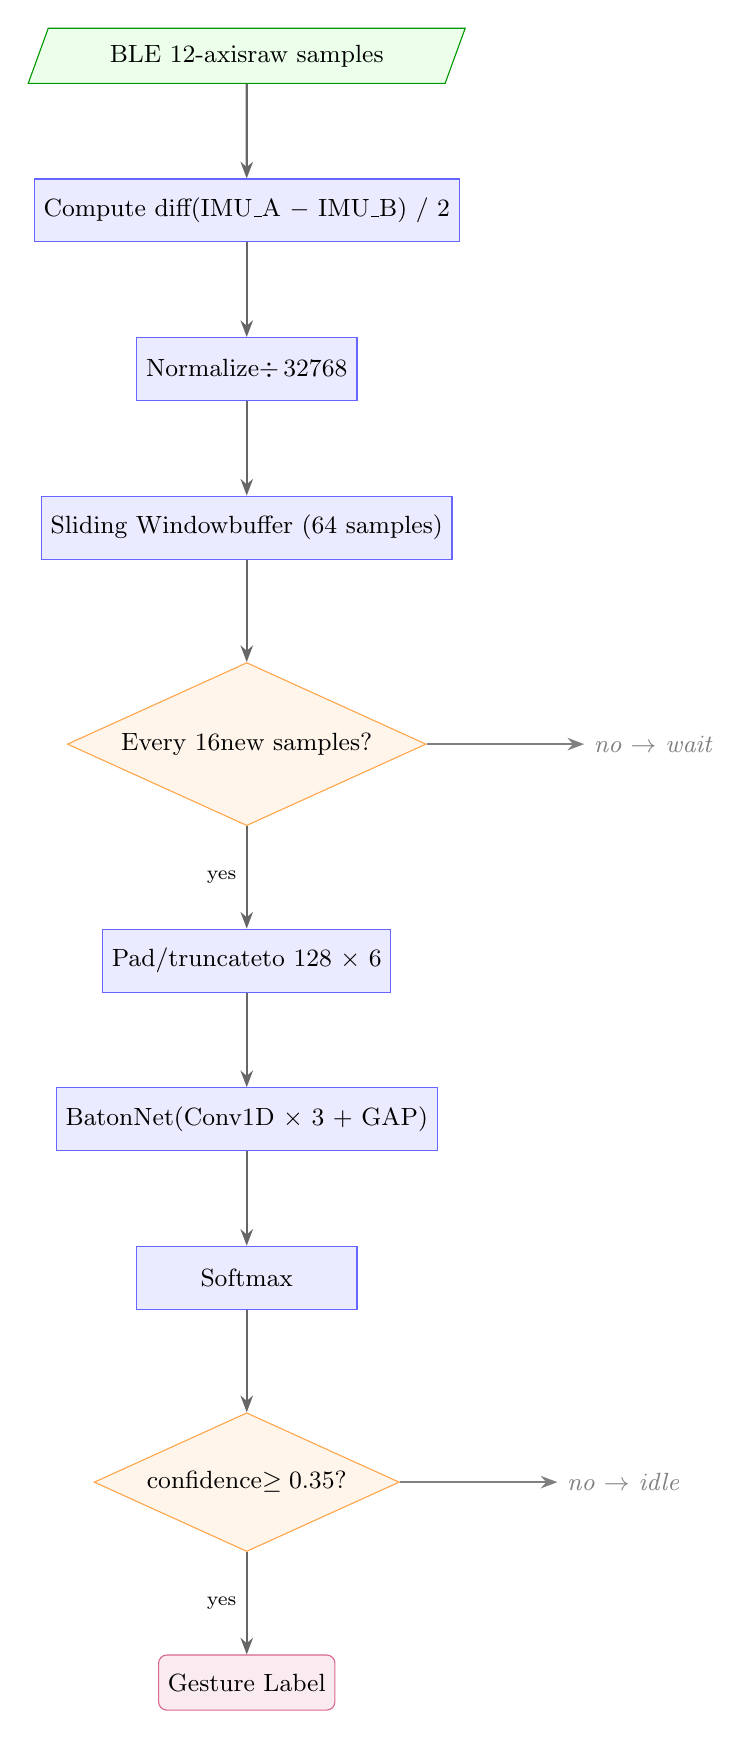
\begin{tikzpicture}[node distance=1.2cm]
  \node[io] (ble) {BLE 12-axis\\raw samples};
  \node[process, below=of ble] (diff) {Compute diff\\(IMU\_A $-$ IMU\_B) / 2};
  \node[process, below=of diff] (norm) {Normalize\\$\div\,32768$};
  \node[process, below=of norm] (buf) {Sliding Window\\buffer (64 samples)};
  \node[decision, below=1.3cm of buf] (stride) {Every 16\\new samples?};
  \node[process, below=1.3cm of stride] (pad) {Pad/truncate\\to 128 $\times$ 6};
  \node[process, below=of pad] (model) {BatonNet\\(Conv1D $\times$ 3 + GAP)};
  \node[process, below=of model] (soft) {Softmax};
  \node[decision, below=1.3cm of soft] (conf) {confidence\\$\geq 0.35$?};
  \node[data, below=1.3cm of conf] (out) {Gesture Label};

  \node[right=2cm of stride, font=\small\itshape, gray] (w1) {no $\rightarrow$ wait};
  \node[right=2cm of conf, font=\small\itshape, gray] (w2) {no $\rightarrow$ idle};

  \draw[arr] (ble) -- (diff);
  \draw[arr] (diff) -- (norm);
  \draw[arr] (norm) -- (buf);
  \draw[arr] (buf) -- (stride);
  \draw[arr] (stride) -- node[left, font=\scriptsize]{yes} (pad);
  \draw[arr] (pad) -- (model);
  \draw[arr] (model) -- (soft);
  \draw[arr] (soft) -- (conf);
  \draw[arr] (conf) -- node[left, font=\scriptsize]{yes} (out);
  \draw[arr, gray] (stride) -- (w1);
  \draw[arr, gray] (conf) -- (w2);
\end{tikzpicture}
\end{center}

% ════════════════════════════════════════════
% Text Summary
% ════════════════════════════════════════════
\newpage
\section{Summary}

\subsection{Hardware}
The baton contains an ESP32 microcontroller and two MPU6050 IMUs (addresses \texttt{0x68} and \texttt{0x69}). It streams 12-axis data (accelerometer + gyroscope $\times$ 2 IMUs) at $\sim$50\,Hz over BLE.

\subsection{Data Collection (\texttt{record.py})}
A Tkinter GUI connects to the baton via BLE, displays real-time waveforms, and records labeled gesture segments as CSV files. Each recording captures one gesture repetition with precise start/stop timing.

\subsection{Training (\texttt{train.py})}
\textbf{BatonNet} is a lightweight 1D-CNN with 3 convolutional layers (24 $\to$ 48 $\to$ 64 channels), batch normalization, max pooling, global average pooling, and a fully-connected classifier. Input is the IMU difference signal (IMU\_A $-$ IMU\_B), normalized and padded to $128 \times 6$. It classifies 8 gestures: idle, beat, stab, spin, slash, shake, flick, wing.

\subsection{Real-Time Detection (\texttt{detect.py})}
A sliding window (64 samples, stride 16) continuously feeds the trained BatonNet model. No energy gating is used --- the model itself distinguishes idle from active gestures. A 0.2\,s cooldown prevents duplicate triggers.

\subsection{Dashboard (\texttt{index.html} + \texttt{server.py})}
\texttt{server.py} connects to the baton via BLE and bridges data to the browser over WebSocket. The dashboard provides:
\begin{itemize}[nosep]
  \item Real-time IMU waveform visualization (accelerometer, gyroscope, magnitude)
  \item Beat detection via jerk thresholding with rising-edge detection and cooldown
  \item BPM estimation from recent beat intervals (sliding window of last 4)
  \item Dynamics classification (\textit{pp} to \textit{ff}) based on jerk magnitude
  \item Integrated MIDI player with 12 embedded classical pieces
  \item Tempo synchronization: baton BPM drives MIDI playback speed in real time, with smooth ramping (0.15\,s follow, 1.0\,s return to original)
  \item Generative visual effects (particles, rings, trails) responding to beat intensity and direction
\end{itemize}

\end{document}
